\documentclass[11pt]{article}

\usepackage[margin=1.1in]{geometry}
\usepackage{amsmath,amssymb,amsthm}
\usepackage{mathtools}
\usepackage{booktabs}
\usepackage{tikz}
\usetikzlibrary{arrows.meta,positioning}
\usepackage{xcolor}
\usepackage{enumitem}
\usepackage[colorlinks=true,linkcolor=blue!60!black,citecolor=blue!60!black,urlcolor=blue!60!black]{hyperref}
\usepackage{microtype}

\newtheorem{theorem}{Theorem}[section]
\newtheorem{lemma}[theorem]{Lemma}
\newtheorem{definition}[theorem]{Definition}
\newtheorem{example}[theorem]{Example}
\newtheorem{claim}[theorem]{Claim}
\newtheorem{openq}[theorem]{Open Question}
\newtheorem*{finding}{Finding}

% Paper-style notation
\newcommand{\vis}{\xrightarrow{\mathsf{vis}}}
\newcommand{\rc}{\xrightarrow{\mathsf{rc}}}
\newcommand{\lo}[1]{\xrightarrow{\mathsf{lo}_{#1}}}
\newcommand{\loC}{\xrightarrow{\mathsf{lo}_{C}}}
\newcommand{\comm}{\rightleftarrows}
\newcommand{\ncomm}{\not\rightleftarrows}
\newcommand{\add}{\mathsf{add}}
\newcommand{\rem}{\mathsf{rem}}
\newcommand{\Merge}{\mathsf{merge}}
\newcommand{\Sinit}{\sigma_0}
\newcommand{\seq}[1]{#1}
\newcommand{\loE}[1]{\mathsf{lo}^{#1}}
\newcommand{\co}{\mathsf{CoreVCs}}
\newcommand{\jp}{\mathsf{JoinPeelVCs}}
\newcommand{\lean}[1]{\texttt{#1}}

\title{\bfseries Set-Relative Linearization and the Join Lemma:\\
\large repairing the verification conditions for bottom-up linearization of
replicated data types, with a machine-checked soundness bridge}
\author{Sal metatheory note\\ \small FP Launchpad, IIT Madras}
\date{July 2, 2026}

\begin{document}
\maketitle

\begin{abstract}
\noindent
The Neem proof methodology reduces RA-linearizability of a replicated data
type (RDT) to a fixed catalogue of \emph{verification conditions} (VCs) ---
equations over $\mathsf{do}$, $\Merge$ and the conflict-resolution relation
$\mathsf{rc}$ --- discharged per data type, with a once-and-for-all
meta-theorem: \emph{if the VCs hold, every reachable configuration is
RA-linearizable}. While mechanising this meta-theorem in Lean~4 we found
that its central induction, \emph{bottom-up linearization}, is unsound as
written: a key step silently assumes a convergence property of
\emph{sub-histories} that is false, and there are reachable configurations
of the paper's own flagship example (the add-wins set) on which \emph{no}
bottom-up peel exists. We further show that no repair by unconditional
equations is possible: the fragment of the VCs that the proof machinery
actually consumes admits a model in which the required peel identities
fail.

This note explains the failure with worked examples, presents the repair
--- a \emph{set-relative} linearization order $\loE{E}$, \emph{canonical
states} $\sigma(E)$, and a single new pair of \emph{contextual}
verification conditions ($\jp$) from which the whole meta-theorem follows
--- and reports on the mechanization: an end-to-end, zero-\lean{sorry}
Lean~4 proof that $\co + \jp$ implies RA-linearizability of every reachable
configuration, together with complete discharges of $\jp$ for the
commuting class of RDTs and for the add-wins set skeleton, i.e.\ exactly
the class of instances on which the original proof breaks.
\end{abstract}

\section{Introduction}

The Neem paper proposes an appealing division of labour for verifying
replicated data types. The \emph{hard, global} property ---
RA-linearizability: every replica's state is explained by a
linearization of the events it has observed, consistent with a
linearization order $\mathsf{lo}$ --- is proved \emph{once}, generically,
from a catalogue of \emph{local, equational} verification conditions:
commutativity and idempotence of $\Merge$, interchange laws between
$\mathsf{do}$ and $\Merge$ (the ``bottom-up'' rules), and coherence
conditions on the conflict-resolution relation $\mathsf{rc}$
(\textsc{rc-non-comm}, \textsc{no-rc-chain}, \textsc{cond-comm}). Each
concrete RDT then only has to discharge the catalogue --- a finite,
SMT-friendly proof obligation.

The generic half of this contract is the \emph{bottom-up linearization}
theorem: given linearization witnesses for the two sides of a merge,
construct one for the merged replica by repeatedly \emph{peeling} a final
event through $\Merge$ using the interchange VCs. We undertook a full
mechanization of this theorem in Lean~4 (over a two-way-merge CRDT
specialization of the model, where the LCA of the paper's three-way merge
collapses to $\Sinit$). The mechanization succeeded in reducing the entire
theorem to the merge case, and then \emph{failed} to close the merge case
--- not for want of automation, but because the paper's argument is
unsound at two points, and because the natural repair lemma turns out to
be \emph{false}. Concretely:

\begin{enumerate}[leftmargin=2em]
\item The proof of the merge case repeatedly asserts that a replica's
witness can be re-ordered to end in a chosen event (``\emph{since $v_i$ is
linearizable, there would exist sequences \ldots\ such that $e_i$ would
appear at the end}''). This conflates the existence of a
\emph{permutation} extending $\mathsf{lo}_C$ with the existence of a
\emph{state-correct witness}: the paper's convergence lemma applies only
to the full event set $E_C$, not to sub-histories, and for sub-histories
the statement is \textbf{false} (Example~\ref{ex:absorber}).
\item There are reachable configurations of the add-wins set on which
\emph{every} choice of final event is blocked: the events that may
legally end the merged witness cannot end either side's witness, and vice
versa (Example~\ref{ex:defeater}). Bottom-up peeling --- with any of the
paper's \textsc{BottomUp-0/1/2-OP} rules, in any order --- cannot
construct the witness, even though the witness exists.
\item No unconditional equation can fill the gap. The general peel
identity that the induction needs is false as a $\forall$-state equation
for the two-key OR-set (Example~\ref{ex:twokey}); and the fragment of the
VCs that the proof machinery actually consumes ($\co$, below) admits a
model --- a ``phantom-conflict'' merge --- that satisfies every VC yet
violates the peel (Example~\ref{ex:phantom}). The gap is therefore
\emph{semantic}, not a missing algebraic law; in particular, the
counter-model is non-associative, isolating associativity of $\Merge$ as
load-bearing.
\end{enumerate}

The repair has three ingredients, each of independent interest:

\begin{itemize}[leftmargin=2em]
\item \textbf{A set-relative linearization order} $\loE{E}$
(Definition~\ref{def:loE}): the overwriter (``absorber'') clause of
$\mathsf{lo}_C$ must range over the event set $E$ of \emph{the version
being linearized}, not over the whole configuration. $\loE{E}$ contains
$\mathsf{lo}_C$ pointwise (so the strengthened witnesses still satisfy
the paper's definition), it is \emph{stable} (independent of the ambient
configuration), and --- decisively --- \textbf{convergence over $E$ holds
with no closure hypotheses at all} (Theorem~\ref{thm:convon}).
\item \textbf{Canonical states and the Join Lemma}
(\S\ref{sec:join}): convergence makes every finite event set $E$ denote a
unique state $\sigma(E)$. The entire meta-theorem then collapses to one
state-level statement,
$\sigma(E_1 \cup E_2) = \Merge(\sigma(E_1), \sigma(E_2))$,
and witness lists disappear from the induction.
\item \textbf{Two contextual verification conditions} ($\jp$,
Definition~\ref{def:jp}): the peel identities that the Join Lemma's
induction consumes, stated \emph{with their context} (maximality of the
peeled event in $\loE{E_1\cup E_2}$, backward closure of the sides). We
prove the Join Lemma, and from it end-to-end RA-linearizability, from
$\co + \jp$ (Theorem~\ref{thm:main}); and we discharge $\jp$ both for the
commuting class and for the add-wins skeleton --- the latter covering
precisely the configurations of Example~\ref{ex:defeater}.
\end{itemize}

Everything above except Example~\ref{ex:phantom} is machine-checked in
Lean~4 with zero \lean{sorry}s (\S\ref{sec:mech}). We close with precise
erratum guidance and the sharpened open question: does $\co$ plus
associativity of $\Merge$ imply $\jp$?

\section{Background, in brief}
\label{sec:background}

We recall only what the examples need, in the paper's notation,
specialized to two-way (state-based CRDT) merge: the LCA of the paper's
three-way $\Merge(l,a,b)$ collapses to $\Sinit$, and a configuration is
$C = \langle N, L, \mathsf{vis}\rangle$ with per-replica states $N(r)$,
per-replica event sets $L(r)$, and a visibility relation $\mathsf{vis}$
over events. Events are triples $e = (t, r, o)$ of a globally fresh
timestamp, an origin replica and an operation; $e(\sigma)$ denotes
$\mathsf{do}(\sigma, e)$ and $\pi(\sigma)$ the left-to-right fold of a
sequence. Two events \emph{commute}, $e_1 \comm e_2$, if
$e_1(e_2(\sigma)) = e_2(e_1(\sigma))$ for every $\sigma$.

\begin{definition}[Linearization relation, {Neem Def.~lin-relation}]
\label{def:loC}
$e_1 \loC e_2$ iff
\[
(e_1 \vis e_2 \;\wedge\; e_1 \ncomm e_2)
\;\;\vee\;\;
\bigl(e_1 \parallel_C e_2 \;\wedge\; e_1 \rc e_2 \;\wedge\;
\neg\exists e_3 \in E_C.\; e_2 \vis e_3 \wedge e_2 \ncomm e_3\bigr).
\]
\end{definition}
The second disjunct is the subtle one: a concurrent non-commuting pair is
ordered by $\mathsf{rc}$ \emph{unless} the target $e_2$ is already
``overwritten'' by a later non-commuting event $e_3$ --- we call such an
$e_3$ an \emph{absorber} of $e_2$. Crucially, the absorber is sought in
the \emph{whole configuration} $E_C$.

A configuration is \emph{RA-linearizable} if every replica $r$ admits a
sequence $\pi$ of exactly the events $L(r)$ such that $\pi$ extends
$\mathsf{lo}_C\restriction_{L(r)}$ and $N(r) = \pi(\Sinit)$. The paper's
convergence lemma states: any two sequences \emph{over $E_C$} extending
$\mathsf{lo}_C$ produce the same state --- the proof uses
\textsc{cond-comm} to swap unordered non-commuting pairs \emph{past an
absorber that the sequence is guaranteed to contain}.

\paragraph{The running data type.}
All examples use the \emph{add-wins skeleton} \textsf{AWSet} (one implicit
key; the mechanized object):
\[
\Sigma = 2^{\mathbb{T}} \times 2^{\mathbb{T}}, \qquad
\Sinit = (\emptyset,\emptyset), \qquad
\sigma = (A, D) \text{ with \emph{live} set } A \setminus D,
\]
\[
\add_t(A,D) = (A \cup \{t\},\, D), \qquad
\rem(A,D) = (A,\, A \cup D), \qquad
\Merge \text{ componentwise } \cup .
\]
A remove kills everything \emph{currently added} --- the state-dependence
is what makes $\add \ncomm \rem$ --- and $\rem \rc \add$ (add wins over a
concurrent remove), exactly the paper's OR-set resolution policy. All 24
paper VCs, including \textsc{cond-comm}, hold for \textsf{AWSet}: a
trailing $\rem$ erases any $\add$/$\rem$ ordering ambiguity, which is
\textsc{cond-comm}'s content.

\section{Three cracks in bottom-up linearization}
\label{sec:cracks}

\subsection{Convergence fails for sub-histories: absorber cancellation}

\begin{example}[The absorber-cancellation configuration]
\label{ex:absorber}
Replica $p$ executes $a = \add_1$ and then $r_p = \rem$ (so $a \vis r_p$).
Replica $q$, concurrently, executes $r_q = \rem$; and $q$ merges $p$'s
state \emph{between} $a$ and $r_p$. So
\[
L(q) = \{r_q,\, a\}, \qquad E_C = \{a,\, r_p,\, r_q\}.
\]

\begin{center}
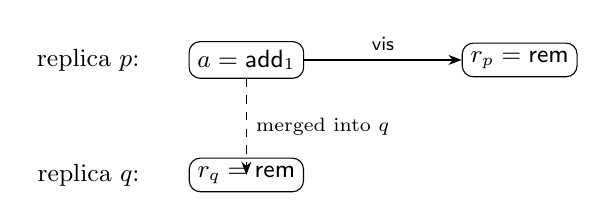
\begin{tikzpicture}[>=Stealth, node distance=1.5cm and 2.0cm,
  ev/.style={draw, rounded corners, inner sep=3pt, font=\small}]
\node[ev] (a) {$a=\add_1$};
\node[ev, right=of a] (rp) {$r_p=\rem$};
\node[ev, below=1.0cm of a] (rq) {$r_q=\rem$};
\node[left=0.5cm of a, font=\small] {replica $p$:};
\node[left=0.5cm of rq, font=\small] {replica $q$:};
\draw[->] (a) -- node[above,font=\scriptsize]{$\mathsf{vis}$} (rp);
\draw[->, dashed] (a) -- node[right,font=\scriptsize]{merged into $q$} (rq -| a) ;
\end{tikzpicture}
\end{center}

What is $\mathsf{lo}_C$ on $L(q) = \{r_q, a\}$? The candidate edge is the
$\mathsf{rc}$ disjunct $r_q \loC a$ (they are concurrent and
$\rem \rc \add$). But $a$ has an absorber \emph{in the configuration}:
$a \vis r_p$ and $a \ncomm r_p$. The clause
``$\neg\exists e_3 \in E_C\ldots$'' therefore \emph{cancels} the edge:
\textbf{$\mathsf{lo}_C$ orders nothing in $L(q)$}. Both orders of $L(q)$
extend $\mathsf{lo}_C\restriction_{L(q)}$, yet
\[
r_q \cdot a\,(\Sinit) = (\{1\}, \emptyset)
\qquad\neq\qquad
a \cdot r_q\,(\Sinit) = (\{1\}, \{1\}).
\]
Only the first is $q$'s actual state (add-wins: the concurrent remove
loses). \emph{Convergence over the sub-history $L(q)$, with respect to
$\mathsf{lo}_C$, is false} --- even though $L(q)$ is causally
(backward-)closed, and even though \textsf{AWSet} satisfies every paper
VC. \hfill$\blacksquare$
\end{example}

Where does the paper use sub-history convergence? In the Merge case of
its main induction, twice over. First, it asserts a \emph{stability
claim}: ``$\mathsf{lo}$ between two events should remain the same in all
versions'' (appendix, Merge case). Example~\ref{ex:absorber} refutes the
forward direction: within $q$'s version, the order $r_q$-before-$a$ is
semantically forced, but in the full configuration the edge is cancelled
by $p$'s local absorber $r_p$ --- a shared event \emph{gains} absorbers
from the other branch. Second, the induction repeatedly re-orders a
side's witness to end in a chosen event $e_i$, justifying the state
equality by linearizability of that version. The justification would
require convergence over that version's event set --- exactly the false
statement. The mechanization surfaced this as an unprovable goal with a
satisfiable context; Example~\ref{ex:absorber} is its counter-model,
machine-checked as
\lean{convergence\_over\_backward\_closed\_subsets\_false}.

\subsection{A reachable configuration that defeats every peel}

One might hope the flaw is local: choose the peeled event more carefully,
re-order less aggressively. The next example closes that door.

\begin{example}[The defeater]
\label{ex:defeater}
One key, four events, three replicas (the third only ferries states).
Replica $p$: $A_p = \add_s$, then $R_p = \rem$. Replica $q$:
$A_q = \add_u$, then $R_q = \rem$. The ferry delivers $A_p$ to $q$
\emph{after} $R_q$, and $A_q$ to $p$ \emph{after} $R_p$:
\[
L(p) = \{A_p, R_p, A_q\}, \qquad L(q) = \{A_q, R_q, A_p\}.
\]
Both sides are backward-closed; the configuration is reachable in five
steps. The replica states are
\[
N(p) = (\{s,u\}, \{s\}) \;\text{(live } u\text{)}, \qquad
N(q) = (\{s,u\}, \{u\}) \;\text{(live } s\text{)},
\]
\[
\Merge(N(p),N(q)) = (\{s,u\},\{s,u\}) \;\text{(live } \emptyset\text{)}.
\]

\begin{center}
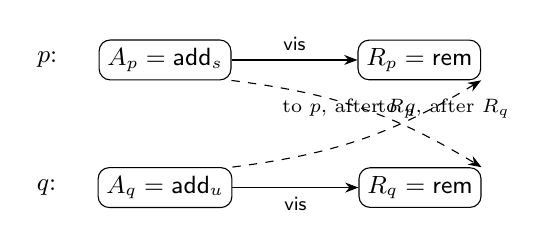
\begin{tikzpicture}[>=Stealth, node distance=0.9cm and 1.6cm,
  ev/.style={draw, rounded corners, inner sep=3pt, font=\small}]
\node[ev] (Ap) {$A_p=\add_s$};
\node[ev, right=of Ap] (Rp) {$R_p=\rem$};
\node[ev, below=1.1cm of Ap] (Aq) {$A_q=\add_u$};
\node[ev, right=of Aq] (Rq) {$R_q=\rem$};
\node[left=0.4cm of Ap, font=\small] {$p$:};
\node[left=0.4cm of Aq, font=\small] {$q$:};
\draw[->] (Ap) -- node[above,font=\scriptsize]{$\mathsf{vis}$} (Rp);
\draw[->] (Aq) -- node[below,font=\scriptsize]{$\mathsf{vis}$} (Rq);
\draw[->, dashed] (Ap.south east) to[bend left=12]
  node[right,font=\scriptsize]{\;to $q$, after $R_q$} (Rq.north east);
\draw[->, dashed] (Aq.north east) to[bend right=12]
  node[pos=0.8, left,font=\scriptsize]{to $p$, after $R_p$\;} (Rp.south east);
\end{tikzpicture}
\end{center}

\emph{Every state-correct witness of $N(p)$ ends in $A_q$.} Indeed
$\mathsf{lo}_C$ on $L(p)$ mandates only $A_p$ before $R_p$ (the edge
$R_p \loC A_q$ is cancelled by the global absorber $R_q$), so three
orders are admissible --- but only $A_p\, R_p\, A_q$ folds to $N(p)$;
placing $A_q$ before $R_p$ kills $u$. Symmetrically every witness of
$N(q)$ ends in $A_p$.

\emph{Every merged witness ends in $R_p$ or $R_q$.} On
$E = L(p) \cup L(q)$, both cross rc-edges are absorber-cancelled, so
$\mathsf{lo}_C = \{A_p \to R_p,\, A_q \to R_q\}$; the maximal events are
the two removes. (E.g.\ $A_p\,R_p\,A_q\,R_q$ folds to
$\Merge(N(p),N(q))$ --- the theorem is \emph{true} here.)

Now consider any bottom-up derivation. Its last step must peel the merged
witness's final event:
\begin{itemize}[leftmargin=2em]
\item peeling $A_q$ or $A_p$ (the sides' actual last events) is illegal
--- they carry live $\mathsf{lo}_C$-edges to $R_q$, $R_p$;
\item peeling $R_p$ or $R_q$ requires the owning side's state to factor
as $e(\,\cdot\,)$ --- but \emph{no} witness of $N(p)$ ends in $R_p$, and
no witness of $N(q)$ ends in $R_q$: the removes are \emph{buried}.
\end{itemize}
The paper's own selection (Merge case, Case~2) picks exactly the buried
event: with $L_\top = \{A_p, A_q\}$, the locals are
$L^a_p = \{R_p\}$, $L^a_q = \{R_q\}$; the induction chooses
$e_1 = R_p$, asserts a witness of $N(p)$ ending in $R_p$ exists ---
false --- and applies \textsc{BottomUp}. \emph{No ordering of the
paper's rules avoids this}: 0-OP needs both sides to end in the same
shared event ($A_q$ vs.\ $A_p$); 1/2-OP need a side's true last event to
be appendable. The induction is stuck on a reachable, VC-satisfying,
four-event instance of the paper's flagship RDT. \hfill$\blacksquare$
\end{example}

\subsection{Why no unconditional equation can help}

During mechanization a ``missing VC'' had been conjectured to bridge such
gaps: a shared-event peel
$\Merge(o_1(\mathit{ol}(a)),\, \mathit{ol}(b)) =
o_1(\Merge(\mathit{ol}(a), \mathit{ol}(b)))$
quantified over \emph{all} states. It is \textbf{false} for
\textsf{AWSet}: take $a = \Sinit$, $b = (\{2\},\emptyset)$,
$\mathit{ol} = \add_1$, $o_1 = \rem$. On the left, the remove cannot see
$b$'s live element $2$; on the right, applied after the merge, it kills
it. (Machine-checked: \lean{AWSet\_shared\_peel\_1op\_false}.) Worse, the
same shape of failure afflicts the \emph{general} peel that the induction
really needs:

\begin{example}[Two keys: contextuality is essential]
\label{ex:twokey}
In a two-key OR-set let $e_1 = \rem_k$ and $e_2 = \add_j$ with
$j \neq k$; they \emph{commute}, so the candidate unconditional rule
``$e_1 \rc e_2 \vee e_1 \comm e_2$ implies
$\Merge(e_1(a), e_2(b)) = e_1(\Merge(a, e_2(b)))$''
(the paper's \textsc{BottomUp-2-OP} premise) applies. Let $b$ hold a live
$k$-element that $a$ has never seen. The left side leaves it alive; the
right side's $\rem_k$, applied after the merge, kills it. The rule is
false as a $\forall$-state equation --- \emph{yet it is exactly what the
induction needs, and it is true in context}: when $e_1$ is about to be
peeled \emph{last}, maximality of $e_1$ in the linearization order of the
\emph{union} guarantees that every non-commuting element of the other
side is either causally ordered against $e_1$ (excluded by backward
closure) or already absorbed on its own side --- so the ``surprise live
$k$-element'' cannot exist. The peel identities are inherently
\emph{contextual}. \hfill$\blacksquare$
\end{example}

\section{The repair: set-relative linearization}
\label{sec:repair}

\subsection{The order $\loE{E}$ and convergence without closure}

Example~\ref{ex:absorber} pinpoints the wrong quantifier in
Definition~\ref{def:loC}: the absorber of $e_2$ must be visible \emph{to
the version being linearized}. (The paper's own Merge-case reasoning
already works with ``$\exists e'' \in L(v_i)$'' --- the corrected
definition makes that official.)

\begin{definition}[Set-relative linearization]
\label{def:loE}
For an event set $E$,\; $e_1 \xrightarrow{\loE{E}} e_2$ iff
\[
(e_1 \vis e_2 \wedge e_1 \ncomm e_2)
\;\vee\;
\bigl(e_1 \parallel e_2 \wedge e_1 \rc e_2 \wedge
\neg\exists e_3 \in E.\; e_2 \vis e_3 \wedge e_2 \ncomm e_3\bigr).
\]
\end{definition}

Three easy but consequential facts (all machine-checked):
\emph{(monotone)} $\mathsf{lo}_C \subseteq \loE{E}$ pointwise --- fewer
absorbers, more edges --- so a witness respecting $\loE{E}$ satisfies the
paper's Def.~lin unchanged, and $E \subseteq E'$ gives
$\loE{E'} \subseteq \loE{E}$ on $E$;
\emph{(stable)} $\loE{E}$ mentions only $\mathsf{vis}$, $\mathsf{rc}$,
$\comm$ restricted to $E$, hence never changes as the configuration
grows --- it is a genuine per-version invariant;
\emph{(acyclic)} $\loE{E}$ has no cycles on $E$: an rc-edge followed by
any edge out of its target dies (a $\mathsf{vis}$-successor \emph{is} an
absorber in $E$; an rc-successor violates \textsc{no-rc-chain}), so
cycles would be pure-$\mathsf{vis}$, contradicting reachability.

In Example~\ref{ex:absorber}, $\loE{L(q)}$ \emph{keeps} the edge
$r_q \to a$ (no absorber of $a$ inside $L(q)$): the fold-wrong order is
excluded, and this is fully general:

\begin{theorem}[Convergence, set-relative --- \lean{convergence\_on}]
\label{thm:convon}
For any finite $E$, any two enumerations of $E$ respecting $\loE{E}$ fold
to the same state, from any starting state. \emph{No overwriter- or
forward-closure hypotheses are required.}
\end{theorem}

\noindent The proof is the paper's bubble-sort argument with one twist
that makes it self-sufficient: whenever two adjacent unordered
non-commuting events must be swapped, the \emph{failure} of the
$\loE{E}$-edge between them hands us an absorber \emph{inside $E$} ---
by definition --- positioned later in both sequences (its
$\mathsf{vis}$-edge from the victim is mandatory); \textsc{cond-comm}
then absorbs the swap. The paper's convergence lemma over $E_C$ becomes
the special case $E = E_C$.

\subsection{Canonical states and the Join Lemma}
\label{sec:join}

Theorem~\ref{thm:convon} makes every finite event set \emph{denote a
state}:

\begin{definition}[Canonical states]
$\sigma(E)$ is the fold of any (hence every) $\loE{E}$-respecting
enumeration of $E$.
\end{definition}

Canonical states enjoy exactly the algebra the induction needs, now as
theorems rather than wishes (each machine-checked):
\begin{itemize}[leftmargin=2em]
\item \textbf{(peel --- \lean{isCanonicalState\_peel})} if $e$ is
$\loE{E}$-maximal then $\sigma(E) = e(\sigma(E\setminus\{e\}))$ --- the
\emph{sound} replacement for the paper's broken re-ordering step: moving
$e$ to the tail and re-sorting the front against
$\loE{E\setminus\{e\}}$ is fold-preserving because the only absorber the
re-sort can lose is $e$ itself, which is applied last;
\item \textbf{(extend --- \lean{isCanonicalState\_extend})} a fresh event
that observed all of $E$ appends: $\sigma(E \cup \{e\}) = e(\sigma(E))$
--- the Apply case;
\item \textbf{(Def-lin)} the canonical enumeration respects
$\mathsf{lo}_C$, so ``replica $r$ holds $\sigma(L(r))$'' implies the
paper's RA-linearizability verbatim.
\end{itemize}

The entire Merge case then collapses to a single state-level statement in
which witness sequences no longer appear:

\begin{definition}[Join Lemma]
For backward-closed $E_1, E_2$ of a reachable configuration:
\[
\sigma(E_1 \cup E_2) \;=\; \Merge\bigl(\sigma(E_1),\, \sigma(E_2)\bigr).
\]
\end{definition}

Note how the Join Lemma dissolves Example~\ref{ex:defeater}: the buried
remove $R_p$ \emph{is} peelable at the $\sigma$-level, because
\[
\Merge(N(p), N(q)) = R_p\bigl(\Merge(\sigma(\{A_p, A_q\}),\, N(q))\bigr)
\]
holds even though $N(p) \neq R_p(\sigma(\{A_p, A_q\}))$ --- the merge
itself supplies the absorber ($R_q$) that $p$'s side lacks. Peeling
through the \emph{join} is strictly more powerful than peeling through a
side.

\subsection{The new verification conditions}
\label{sec:newvcs}

Which VCs does this machinery consume? Auditing the mechanized proofs
yields a seven-field fragment we call $\co$:
\textsc{rc-non-comm} (directional), \textsc{no-rc-chain},
\textsc{cond-comm} (lifted across an intervening sequence),
$\Merge$-commutativity, $\Merge(\Sinit, s) = s$, the two-sided shared
peel $\Merge(e(a), e(b)) = e(\Merge(a,b))$, and the all-commuting peel.
(The audit matters: \textsf{AWSet} \emph{cannot} satisfy the previously
extended bundle --- the false shared-peel VC above --- so the generic
theory must be parameterized by the fragment.)

The Join Lemma's induction --- select a $\loE{E_1\cup E_2}$-maximal
event, peel, recurse --- is then fully generic \emph{except} for two
state equations, which Example~\ref{ex:twokey} shows cannot be
unconditional. We therefore state them \emph{with their context}:

\begin{definition}[$\jp$]
\label{def:jp}
For all reachable $C$, backward-closed $E_1, E_2$, and $e$ maximal in
$\loE{E_1 \cup E_2}$:
\begin{align*}
\textsc{peel-local}:&\quad e \in E_1 \setminus E_2 \;\Rightarrow\;
\Merge(\sigma(E_1), \sigma(E_2)) =
e\bigl(\Merge(\sigma(E_1{\setminus}\{e\}),\, \sigma(E_2))\bigr),\\[2pt]
\textsc{peel-shared}:&\quad e \in E_1 \cap E_2 \;\Rightarrow\;
\Merge(\sigma(E_1), \sigma(E_2)) =
e\bigl(\Merge(\sigma(E_1{\setminus}\{e\}),\, \sigma(E_2{\setminus}\{e\}))\bigr).
\end{align*}
\end{definition}

\begin{theorem}[Main theorem]
\label{thm:main}
If an RDT satisfies $\co$ and $\jp$, then every configuration reachable
from the initial configuration is RA-linearizable.
\end{theorem}

\noindent\emph{Mechanized as} \lean{ra\_linearizable\_of\_core\_join}.

\noindent The proof is an induction over executions carrying the
strengthened invariant \emph{every replica holds the canonical state of
its event set} (plus transitivity and irreflexivity of $\mathsf{vis}$,
themselves proved as reachable invariants). CreateReplica and Query are
trivial; Apply is \emph{extend} plus a locality observation (a fresh
event's new $\mathsf{vis}$-edges never touch other replicas' sets, so
their canonical witnesses survive --- this is where stability of
$\loE{E}$ pays); Merge is the Join Lemma, proved from $\jp$ by the
maximal-peel induction.

\subsection{Discharging $\jp$: the trichotomy}
\label{sec:discharge}

$\jp$ is a per-RDT obligation, like the original 24. Two complete
discharges are mechanized.

\paragraph{The commuting class.} If all events pairwise commute (G-Set
and its relatives), \textsc{rc-non-comm} makes $\loE{E}$ empty, every
enumeration is canonical, and both peels follow from the all-commuting
peel and the two-sided shared peel. RA-linearizability for this class is
thus unconditional.

\paragraph{\textsf{AWSet}.} Here $\mathsf{rc}$ is non-trivial and the
defeater configurations live. The discharge has two steps, and their
shape is, we believe, the template for real OR-sets and RGAs:

\emph{(1) Characterize $\sigma$.} For every event set,
\[
\sigma(E) = \bigl(\;\mathsf{adds}(E),\;\;
\{\,\text{adds of } E \text{ absorbed \emph{inside} } E\,\}\;\bigr),
\]
proved by a sandwich invariant along any $\loE{E}$-respecting
enumeration: an add absorbed within the processed prefix is already dead
(its $\mathsf{vis}$-edge to the absorber is mandatory), and everything
dead is absorbed within $E$ (a remove can never precede an unabsorbed
concurrent add --- the rc-edge $\rem \to \add$ would be mandatory in
$\loE{E}$). Note how the \emph{set-relative} order makes the
characterization possible at all: with $\mathsf{lo}_C$,
Example~\ref{ex:absorber} shows the fold is not even a function of the
set.

\emph{(2) The trichotomy.} Let $e$ be a $\loE{E_1\cup E_2}$-maximal
remove, $e \in E_1$. For \emph{any} add $x$ of $E_1 \cup E_2$: since
maximality cancels the edge $e \to x$, either
(i) $x \vis e$ --- then $e$ absorbs $x$ and backward closure of $E_1$
puts $x$ beside its absorber; or
(ii) $x$ has an absorber $z$ somewhere in the union --- and since
$x \vis z$, backward closure of \emph{whichever side contains $z$} drags
$x$ there too. Either way \emph{$x$ is absorbed on a side that owns it}:
both sides' dead-sets saturate, and \textsc{peel-local}/\textsc{shared}
reduce to set algebra over the characterization. In
Example~\ref{ex:defeater}: peeling $e = R_q$, the adds $A_p, A_q$ are
absorbed by $R_p \in L(p)$ and $R_q \in L(q)$ respectively --- the merge
equation holds although $q$'s state never factored through $R_q$ last.

\section{The boundary: what cannot be weakened}
\label{sec:boundary}

Could $\jp$ be derived generically from $\co$, making the new conditions
free? No:

\begin{example}[The phantom-conflict merge]
\label{ex:phantom}
Let \textsf{AWSetX} be \textsf{AWSet} with $\mathsf{do}$, $\mathsf{rc}$
unchanged and
\[
\Merge_X\bigl((A_1,D_1),(A_2,D_2)\bigr) =
\Bigl(A_1 \cup A_2,\;\; D_1 \cup D_2 \cup
\underbrace{\bigl[\text{if } D_1 \neq \emptyset \wedge D_2 \neq \emptyset
\text{ then } A_1 \mathbin{\triangle} A_2 \text{ else } \emptyset\bigr]}_{\text{phantom conflict}}\Bigr).
\]
Every field of $\co$ survives the injection. The update-level fields do
not mention $\Merge$. For the rest: commutativity ($\triangle$ is
symmetric) and $\Merge_X(\Sinit, s) = s$ (guard off) are immediate; the
two-sided shared peel holds because a synchronized $\add_t$ leaves the
guard and $A_1 \mathbin{\triangle} A_2$ \emph{invariant}, while a
synchronized $\rem$ pushes both added-sets into dead, \emph{absorbing}
the injection; and the all-commuting peel holds because an add commutes
only with adds, whose fold has empty dead (guard off), and a remove only
with removes, whose fold is $\Sinit$.

Yet \textsc{peel-local} fails. Take $p$: $\add_s$, $\rem$, then
$e = \add_t$ (so $e$ is union-maximal and unabsorbed); $q$: $\add_u$,
$\rem$. Then $\sigma(L(p)) = (\{s,t\},\{s\})$,
$\sigma(L(p){\setminus}\{e\}) = (\{s\},\{s\})$,
$\sigma(L(q)) = (\{u\},\{u\})$, and
\begin{align*}
\Merge_X(\sigma(L(p)), \sigma(L(q))) &= (\{s,t,u\}, \{s,t,u\}), \quad\text{but}\\
e\bigl(\Merge_X(\sigma(L(p){\setminus}\{e\}), \sigma(L(q)))\bigr)
&= (\{s,t,u\}, \{s,u\}) :
\end{align*}
the phantom conflict kills the freshly peeled, unabsorbed add $t$.
\hfill$\blacksquare$
\end{example}

So $\co \not\Rightarrow \jp$: the peel identities are genuinely new
content, not a consequence of the existing equations --- and, a fortiori,
the paper's 24 VCs do not force them either. Two further observations
sharpen the picture. First, a \emph{forcing analysis} shows the freedom
exploited by $\Merge_X$ is exactly the dead-component: any extra
\emph{Boolean} distinction added to the state is provably constant under
$\co$ (crush both sides with a remove, un-crush to an all-adds pair,
strip with the commuting peel, land on $\Merge(\Sinit,\cdot)$), and the
added-component of any $\co$-merge is forced to be the union on all
fold-pairs. Second --- and this is the constructive lead ---
\textbf{$\Merge_X$ is not associative}:
\begin{align*}
\bigl((\{x\},\{x\}) \sqcup (\{y\},\{y\})\bigr) \sqcup (\{z\},\emptyset)
&\;\text{ has dead } \{x,y\}, \quad\text{but}\\
(\{x\},\{x\}) \sqcup \bigl((\{y\},\{y\}) \sqcup (\{z\},\emptyset)\bigr)
&\;\text{ has dead } \{x,y,z\},
\end{align*}
and every associative repair of the injection we attempted collapses.
Associativity of $\Merge$ --- true of every real lattice-based RDT, and
absent from the paper's VC catalogue --- is load-bearing:

\begin{openq}
Does $\co$ together with associativity (and idempotence) of $\Merge$
imply $\jp$? A proof would repair the original meta-theorem at full
generality at the cost of one per-RDT-trivial VC; the phantom-conflict
model shows the question is tight from below.
\end{openq}

\section{The mechanization}
\label{sec:mech}

All results except Example~\ref{ex:phantom} (currently a hand-verified
analysis) are formalized in Lean~4 (v4.28.0, Mathlib) over the Sal
emulation framework, with \textbf{zero \lean{sorry}s} in every file
listed below; the kernel-checked axioms are the standard
\lean{propext}, \lean{Classical.choice}, \lean{Quot.sound}.

\begin{center}
\small
\begin{tabular}{@{}ll@{}}
\toprule
\textbf{Artifact} & \textbf{Content} \\
\midrule
\multicolumn{2}{@{}l}{\emph{File} \lean{Merge\_Linearization\_Set.lean}}\\
\quad $\loE{E}$, monotonicity, acyclicity & Def.~\ref{def:loE} and its theory \\
\quad \lean{convergence\_on} & Theorem~\ref{thm:convon} \\
\quad $\sigma$, peel, extend, normalization & \S\ref{sec:join} \\
\quad $\co$, \lean{JoinPeelVCs}, \lean{join\_lemma\_of\_peel} & the Join Lemma from $\jp$ \\
\quad commuting-class discharge & \S\ref{sec:discharge} \\
\midrule
\multicolumn{2}{@{}l}{\emph{File} \lean{Convergence\_CounterModel.lean}}\\
\quad \textsf{AWSet} + all $\co$ fields & the running RDT \\
\quad Example~\ref{ex:absorber} formalized & sub-history convergence refuted \\
\quad shared-peel VC refuted & \S3.3 \\
\quad $\sigma$-characterization, trichotomy & \S\ref{sec:discharge} \\
\quad \lean{AWSet\_joinPeelVCs}, \lean{AWSet\_joinLemma} & $\jp$ for \textsf{AWSet} \\
\midrule
\multicolumn{2}{@{}l}{\emph{File} \lean{RA\_Lin\_Of\_Join.lean}}\\
\quad \lean{ra\_linearizable\_of\_core\_join} & Theorem~\ref{thm:main}, end-to-end \\
\bottomrule
\end{tabular}
\end{center}

A few proof-engineering notes that may be of independent use.
\emph{(i) Acyclicity without well-foundedness machinery:} maximal
elements of $\loE{E}$ are extracted by a greedy walk over an enumerating
list, with cycles refuted directly (the ``rc-edge followed by anything
dies'' argument); no order-theoretic typeclasses are needed.
\emph{(ii) The normalization lemma} is where the corrected re-ordering
lives: after peeling a tail event $t$, the remaining front need not
respect $\loE{E \setminus \{t\}}$ (edges reappear whose only absorber was
$t$); re-sorting is fold-preserving precisely because both the old and
new fronts, \emph{with $t$ appended}, respect $\loE{E}$, and
Theorem~\ref{thm:convon} applies at $E$. This is the paper's implicit
step, made true. \emph{(iii) The sandwich invariant} for the
\textsf{AWSet} characterization shows a pattern that should transfer to
multi-key OR-sets and RGAs: prove the canonical fold computes a
\emph{configuration-level} function of the event set, then do all peel
reasoning in that image. \emph{(iv) Modularity of VC bundles} turned out
to be essential, not cosmetic: the previously extended bundle is
unsatisfiable for \textsf{AWSet}, so the generic theory is parameterized
by the audited fragment $\co$, with the full bundle recovered as an
instance. \emph{(v) The refuted route is retained}: the original
bottom-up induction, with its six unprovable goals, is kept quarantined
in \lean{Merge\_Linearization.lean} as executable documentation of
\S\ref{sec:cracks}.

\section{Guidance for an erratum, and conclusion}

For the authors of the original proof, the precise repair points are:
\begin{enumerate}[leftmargin=2em]
\item \emph{Case 1.1.2} (commuting sub-case): the cited
\textsc{no-rc-chain} step does not literally apply; a correct argument
exists and is mechanized (\lean{no\_lo\_of\_concurrent\_to\_L\_b}) ---
erratum-sized.
\item \emph{The stability claim} (``$\mathsf{lo}$ remains the same in all
versions''): false in the forward direction
(Example~\ref{ex:absorber}); the correct per-version order is
$\loE{L(v)}$, and only the direction
$\mathsf{lo}_{E_1\cup E_2} \Rightarrow \loE{L(v_i)}$ on $L(v_i)$ survives.
\item \emph{The re-ordering steps} (``there would exist sequences ending
in $e_i$''): unsound as justified; Example~\ref{ex:defeater} defeats
every version of the bottom-up peel. The repair is structural: canonical
states, the Join Lemma, and the contextual conditions $\jp$ ---
\emph{not} a patch to the induction as written.
\item \emph{The VC catalogue} must grow: $\jp$ (or any lattice-level
axioms that imply it --- associativity is the leading candidate) is new
content, unprovable from the existing equations
(Example~\ref{ex:phantom}).
\end{enumerate}

The resulting contract keeps the spirit of the original: a per-RDT,
finite, mostly-equational obligation ($\co$, plus $\jp$ discharged by the
characterize-then-trichotomy pattern), and a once-and-for-all,
machine-checked meta-theorem. The mathematics that emerged --- absorber
cancellation, set-relative orders, canonical states, join-level peeling
--- seems to us the correct abstraction layer for linearizing state-based
replication, and the open question above is now a sharp target: settle
whether associativity closes the gap, or exhibit the separating model
that proves the per-RDT conditions irreducible.

\end{document}
